\chapter{Modelado de sistemas dinámicos}
Warning: Section in progress
\section{Ejemplos}
\subsection{El oscilador de Van der Pol}
Se trata de un oscilador, propuesto por primera vez por Balthasar Van der Pol, cuando trabajaba en Philips, para explicar las oscilaciones observadas en tubos de vacío. Podemos obtener la ecuación del oscilador, empleando el circuito de la figura \ref{fig:vdp}
\begin{figure}
\centering
\begin{circuitikz}[american, scale = 0.6]\draw
(0,-4)to[short]
(4,-4)to[short,,i^<= $i_C$]
(5,-4)to[short,i=$i_N$]
(6,-4)to[short](10,-4)
(0,-7.5)to[C = C](0,-4)
(5,-4) to[L = L, i>^= $i_L$,*-* ](5,-7.5)
(10,-4) to[generic=NL,  i= $i_N \equiv h(v)$](10,-7.5) 
(0,-7.5)to[short](10,-7.5)
;
\end{circuitikz}  
\label{fig:vdp}
\caption{Circuito eléctrico no lineal}
\end{figure}

Donde el elemento no lineal NL, presenta una relación entre voltaje e intensidad caracterizada por la función $h(v)$.

El voltaje $v$ en los tres componentes del circuito debe ser igual; además,
\begin{align}
v = L \frac{di_L}{dt}\\
i_C = C\frac{dv}{dt}
\end{align}
Si aplicamos la primera ley de Kirchohff al nodo superior del circuito,
\begin{align}
i_C+i_L+i_N = 0\\
C\frac{dv}{dt}+\frac{1}{L}\int_{-\infty}^{t}v(s)ds +h(v)=0\label{eq:vdp}
\end{align}
Si derivamos \ref{eq:vdp} con respecto al tiempo, dividimos por $C$ y reordenamos,
\begin{equation}\label{eq:vdp2}
\frac{d^2v}{dt^2}  + \frac{1}{C}\frac{dh(v)}{dv}\frac{dv}{dt} + \frac{1}{LC}\cdot v= 0
\end{equation}
Se trata de un caso particular de la ecuación de Liénard,
\begin{equation}
\ddot{v} +f(v)\dot{v}+g(v) = 0
\end{equation}
Si definimos ahora, $h(v)$,
\begin{align}
h(v) = m(\frac{1}{3}v^3-1)\\
\frac{dh}{dv} = m(v^2-1)
\end{align}
y sustituyendo en \ref{eq:vdp2},
\begin{equation}
\ddot{v} +m\frac{1}{C}(v^2-1)\dot{v}+\frac{1}{LC}v = 0
\end{equation}

Podemos representarla finalmente en variables de estado, tomando $x_1=v$ y $x_2=\dot{v}$,
\begin{align}
\dot{x}_1 &= x_2\\
\dot{x}_2 &= -\frac{1}{LC}x_1 - m\frac{1}{C}(x_1^2-1)x_2 \label{eq:vdpst2}
\end{align}
Podemos ahora hacer un primer análisis cualitativo. El primer término a la derecha del igual en  la ecuación \ref{eq:vdpst2} representa una fuerza recuperadora proporcional al desplazamiento, el segundo término, crecerá con la velocidad para $x_1 < 1$, alejando así al sistema del origen  y representará un término disipativo para $x_1 > 1$ acercándolo por tanto de nuevo al origen. Es por tanto esperable, que se alcance
algún tipo de situación de equilibrio. Más adelante definiremos esta situación rigurosamente como un ciclo límite. 
\subsection{Un vehículo de cuatro ruedas. }
La figura \ref{fig:vehir} muestra un esquema de un vehículo terrestre de cuatro ruedas, visto desde arriba. Si consideramos que se mueve en el plano $x,y$, y que su velocidad instántanea $\vec{V}$ está siempre orientada en la dirección de avance del vehículo $psi$--asumimos que no derrapa, ni se mueve lateralmente--, podemos entoces definir el velocidad, en el sistema de referencia $x,y$ como,
\begin{align}
\dot{x} = V_x(t) = V\cos(\psi(t))\\
\dot{y} = V_y(t) = V\sin(\psi(t))\\
\end{align}

\begin{figure}
\centering

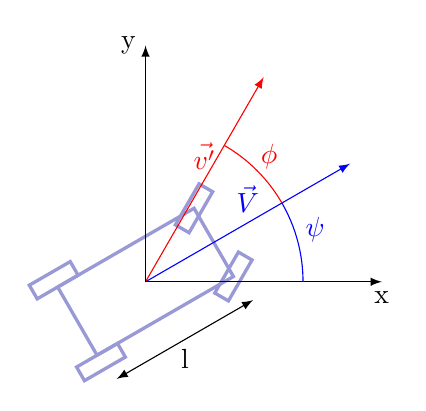
\begin{tikzpicture}
\draw(0,0)[rotate around={30:(0,0)},very thick,draw = blue!60!black!40]rectangle(2,1);
\draw(-0.3,-0.2)[rotate around={30:(0,0)},very thick,draw = blue!60!black!40]rectangle(0.3,0.0);
\draw(-0.3,1)[rotate around={30:(0,0)},very thick,draw = blue!60!black!40]rectangle(0.3,1.2);
\draw({2*cos(30)-0.3},{2*sin(30)-0.1})[rotate around={60:({2*cos(30)},{2*sin(30)})},very thick,draw = blue!60!black!40]rectangle({2*cos(30)+0.3},{2*sin(30)+0.1});
\draw({2*cos(30)-sin(30)-0.3},{2*sin(30)+cos(30)-0.1})[rotate around={60:({2*cos(30)-sin(30)},{2*sin(30)+cos(30)})},very thick,draw = blue!60!black!40]rectangle({2*cos(30)-sin(30)+0.3},{2*sin(30)+cos(30)+0.1});
\draw[blue]({cos(30)-0.5*sin(30)},{sin(30)+0.5*cos(30)})--node[above]{$\vec{V}$}({4*cos(30)-0.5*sin(30)},{4*sin(30)+0.5*cos(30)})[-latex];
\draw[red]({cos(30)-0.5*sin(30)},{sin(30)+0.5*cos(30)})--node[above]{$\vec{v'}$}({cos(30)-0.5*sin(30)+3*cos(60},{sin(30)+0.5*cos(30)+3*sin(60})[-latex];

\draw({cos(30)-0.5*sin(30)},{sin(30)+0.5*cos(30)})--({3+cos(30)-0.5*sin(30)},{sin(30)+0.5*cos(30)})[-latex]node[anchor=north]{x};
\draw({cos(30)-0.5*sin(30)},{sin(30)+0.5*cos(30)})--({cos(30)-0.5*sin(30)},{3+sin(30)+0.5*cos(30)})[-latex]node[anchor=east]{y};

\draw[blue]({2+cos(30)-0.5*sin(30)},{sin(30)+0.5*cos(30)})arc(0:30:2);
\draw[red]({3*cos(30)-0.5*sin(30)},{3*sin(30)+0.5*cos(30)})arc(30:60:2);
\draw[blue]({3.2*cos(30)},{3.2*sin(30)}) node[]{$\psi$};
\draw[red]({3.4*cos(50)},{3.3*sin(50)}) node[]{$\phi$};
\draw[latex-latex](0.25,-0.3)--node[below]{l}({2*cos(30)+0.25},{2*sin(30)-0.3});
\end{tikzpicture}
\label{fig:vehir}
\caption{Esquema de un vehículo terrestre de 4 ruedas}
\end{figure}

Además el vehículo girará, siempre que las ruedas delanteras no estén alineadas con las ruedas traseras, cambiando así su dirección de avance . Podemos relacionar la velocidad de giro del vehículo $\dot{\psi}$ con el ángulo de orientación de las ruedas delanteras $\phi$, y la velocidad a la que avanzan $\vec{v'}$.  podemos obtener las componetes de dicha velocidad en ejes cuerpo (paralela y perpendicular a la dirección de avance del vehículo),

\begin{align}
v_{P} = v'\cos(\phi(t))\\
v_{T} = v'\sin(\phi(t))
\end{align} 

Pero la rueda esta unida al vehículo así que su velocidad en la direccíon de avance debe ser la misma que la del vehículo: $v_P \equiv V$.  A partir de esta relación podemos obtener la velocidad tangencial de las ruedas como,
\begin{equation}
v_T = V\frac{\sin(\phi)}{\cos(\phi)} = V\tan(\phi)
\end{equation}

Si tomamos como centro de giro del vehículo el centro de su eje trasero, y la batalla (distancia entre ejes) es $l$, obtenemos una expresión para su velocidad de giro,
\begin{equation}
\dot{\psi} = \frac{V}{l}\tan(\phi)
\end{equation}

En resumen, podemos describir el sistema mediante tres ecuaciones de estado $x_1 \equiv x, x_2\equiv	y, x_3 \equiv \psi$:
\begin{align}
\dot{x_1} =  V\cos(x_3)\\  
\dot{x_2} =  V\sin(x_3)\\
\dot{x_3} = \frac{V}{l}\tan(\phi)
\end{align}

Si consideramos $V=cte$, la única entrada al sistema sería el ángulo de giro de las ruedas $u(t) = \phi(t)$, controlando su valor, podemos hacer girar al vehículo en la dirección deseada. 
 